% Chapitres/Chap3-UnOutilAideDecision

\itodo{Pourquoi, Comment, quelle utilité ?\\
       Rappeler ce qui différencie cette approche des autres issues de la littérature:\\
       (i) Approche couplée système/enveloppe \\
       (ii)Optimisation complète systèmes/contrôle/enveloppe
}



% ..............................................................................
% ..............................................................................
\section{L’optimisation Multi-objectif} % (fold)
\label{sec:multi_critere}

% ------------------------------------------------------------------------------
\subsection{Introduction} % (fold)
\label{sub:introduction}
\itodo{À reprendre complètement}

L’optimisation multi-objectif est aujourd’hui largement utilisé dans le bâtiment.
On a par exemple \cite{Armand-Decker2015} qui a développé une méthode d’optimisation pour les
construction bois en utilisant un meta-modèle de bâtiment. Elle utilise un meta-heuristique
à population (Particule Swarm optimization) et évalue les besoins en énergie, le confort des
occupants, la sécurité de l’ouvrage et de l’impact environnemental. \cite{Rivallain2013}
a quand à lui utilisé une méthode approchée (NSGA-II) et une exacte (programmation dynamique)
pour identifier des programmes séquentiels efficaces de réhabilitation énergétique.
Il a ainsi optimisé la combinaison des modifications pour chaque phase mais aussi l’ordre
dans lequel ces améliorations doivent être réalisées afin d’être le plus optimal
possible.
Pour les différentes solutions l’impact environnemental, le confort des occupants en
période estivale, et le coût ont été évaluées.
\itodo{Ajouter des sources vers des exemples d’optimisation de bâtiment}

On a aussi de nombreux exemples d’optimisation de système énergétique.
\itodo{Ajouter des sources vers des exemples d’optimisation de système}

On voit donc que l’optimisation est un outil qui a été largement utilisé dans
le bâtiment comme pour l’amélioration ou l’identification de solutions performantes
pour les systèmes.
L’originalité de ce travail provient principalement du couplage entre le bâtiment
et ses systèmes. La plupart des optimisations de bâtiment évalues les besoins
du bâtiment et considère donc un système de chauffage et de ventilation idéaux.
Dans ces travaux on cherche à optimiser la partie système et son algorithme de
contrôle en même temps que l’enveloppe du bâtiment. On évalue donc plus un besoin
en énergie mais une consommation qui est fonction de la performance des systèmes
envisagées. Les travaux se concentre sur l’évaluation de solutions utilisant fortement
l’énergie solaire comme vecteur énergétique. On cherche donc à couvrir les besoins
de chauffage, d’eau chaude sanitaire (ECS) et d’électricité.
Cette approche permettra d’évaluer le potentiel d’autonomie solaire disponible
pour différentes combinaisons systèmes/enveloppe.
\itodo{Ajouter du bla bla sur l’originalité et les perspectives de ces travaux}

Enfin ces travaux vise à l’élaboration d’un outil d’aide à la décision. Il existe
diverses methodes pour faire de l’aide à la décision comme décrites dans le chapitre
précédent~\autoref{sec:multi_critere}. L’approche choisie est de déterminer un
ensemble de solutions non-dominées dans un premier temps, puis d’utiliser des
outils d’aide à la décision pour réduire le nombre de solution. On se trouve donc
dans une approche par front de Pareto.
\itodo{Ajouter du bla bla sur le choix de l’ordre entre optimisation et aide à la décision}

\itodo{Reformuler tout ça pour mieux introduire les parties qui suivent}
% subsection introduction (end)


% ------------------------------------------------------------------------------
\subsection{Les approches existantes} % (fold)
\label{sub:les_approches_existantes}
\itodo{
Description des méthodologies:\\
 - Formulation\\
 - Optimisation puis décision\\
 - Décision puis optimisation\\
 - Combinée
}

\itodo{
Description des méthodes existantes:\\
 - Graphe des possibilités\\
 - Exactes\\
 - Approchées
}

\itodo{
Les type de variables:\\
 - Quantitative\\
 - Qualitative (combinatoire, continue)
}

\itodo{
Approches Pareto:\\
 - Comparaisons de solution\\
 - Front de Pareto\\
 - Critère de performance (Hyper-volume, répartition, convergence, rapidité)\\
 - Les méthode de sélection de Front de Pareto\\
 - les métriques utilisable pour évaluer la qualité de ce front
}
% subsection les_approches_existantes (end)
% section multi_critere (end)




% ..............................................................................
% ..............................................................................
\section{L’analyse de sensibilité} % (fold)
\label{sec:l_analyse_de_sensibilite}

% ------------------------------------------------------------------------------
\subsection{Les méthodes existantes} % (fold)
\label{sub:les_méthodes_existantes}
\itodo{
Nécessiter de limiter le nombre de variables à évaluer pour réduire la cardinalité
du problème.\\
Réduction du nombre de variables par l’étude de sensibilité:\\
 - Méthodes locales\\
 - Méthodes globales\\
 - Screening (Morris)
}
% subsection les_méthodes_existantes (end)

% ------------------------------------------------------------------------------
\subsection{Réduction de la cardinalité par screening} % (fold)
\label{sub:reduction_de_la_cardinalite_par_screening}
\itodo{Présenter l’analyse de sensibilité choisie (graphique, description, ...)}
% subsection reduction_de_la_cardinalite_par_screening (end)
% section l_analyse_de_sensibilite (end)




% ..............................................................................
% ..............................................................................
\section{Construction d’un outil d’aide à la décision} % (fold)
\label{sec:construction_d_un_outil_d_aide_à_la_decision}


% ------------------------------------------------------------------------------
\subsection{Génération de solutions: quelle méthode ?} % (fold)
\label{sub:generation_de_solutions_quelle_methode}
% Description du Meta-heuristique choisi:
%  - Origine de l’algorithme (inspiration des abeilles):
% Décrire l’origine de cet algorithme. Décrire les recherches qui ont été faites sur
% les abeilles et ensuite les conclusions tirées par l’inventeur pour formuler ce
% meta-heuristique.
% Les sources suivantes non pas encore été lues: \cite{Camazine1991547}, \cite{Seeley1996}
% mais traitent du comportement des abeilles.
%  - Formulation théorique:
%     + Description des différentes étape de résolution de la méthode:
%       Détails pour onlookers, employed, scout, ...
%       Détails pour les paramètres nécessaires au fonctionnement de l’heuristique.
%     + Description de la mise à jour de la position d’une source:
%       Dans le cas de variables continues la formulation de base est applicable et sera
%       donc conservée. Dans le cas de variables discrètes on utilisera une méthode alternative
%       développée dans `10.1177/0021998308097681` et `tel-01234197, version 1`.

% - - - - - - - - - - - - - - - - - - - - - - - - - - - - - - - - - - - - - - -
\subsubsection{Quelle approche d’optimisation ?} % (fold)
\label{ssub:quelle_approche_d_optimisation_}
Comme nous l’avons vu précédemment, il existe de nombreux meta-heuristiques dans
la littérature. Cependant il n’existe pas à la connaissance de l’auteur de méthode
pour sélectionner un algorithme qui sera le plus performant pour un problème donnée.
Ce principe a été formalisé par \cite{Wolpert199767} \itodo{Pas encore lu ...}. Il démontre qu’il
n’y a aucunes \emph{à priori} différences entre les algorithmes. Les critères
permettant de sélectionner un meta-heuristique sont donc à caractère subjectif.
Un des arguments pertinent qui peut être mis en avant est le nombre de paramètres
nécessaires pour le réglage de l’algorithme. En effet sur ce point les algorithmes
sont très différents, certains demandant de nombreux paramètres à configurer
\itodo{Citer des exemple de algo génétique, réseaux de neuronnes, ...} contrairement
à d’autres \itodo{Citer des exemples de PSO, ABC, ...}. Un autre critère pertinent
est la robustesse des algorithmes. On entend par \emph{robuste} la capacité des algorithmes
à converger pour différentes valeurs de paramètre. Par exemple le meta-heuristique PSO
peut être considérée comme robuste \itodo{Mettre des sources} car la solution n’est
pas fortement influencée par le choix de la configuration.
À l’opposée des approches par réseau de neurones \itodo{Mettre des sources} sont
très sensibles, et la variation d’un paramètre peut donner une solution complètement
différente (pour le meilleur et le pire).
Afin de pallier à ces problème, des outils existent pour paramétrer ces meta-heuristique.
C’est particulièrement vrai dans le cas d’optimisation mono-critère mais commence
aussi à émerger pour des problème plus complexe. \cite{Lopez-Ibanez2012861}
présente un framework pour faire de l’optimisation multi-objectifs en utilisant
différents algorithmes de colonies de fourmis (MOACO). Il propose aussi un outil
pour configurer automatiquement les paramètres du meta-heuristique en utilisant un jeu de solution
d’entrainement. Pour ce faire les auteurs ont adapté l’algorithme \emph{F-Race} (\cite{Lopez-Ibanez2011})
au problème multi-objectif pour différentes (\cite{Birattari2010311,Zitzler2003117}). Les auteurs montrent
alors que les configurations trouvées automatiquement sont meilleures que celles
de la littérature pour différents type de problèmes. Cette approche permet alors
de se passer de l’étape de configuration manuelle et pourrait si généralisée/généralisable
permettre au meta-heuristique très dépendant de ces paramètres d’être plus simples
à utiliser.
\itodo{Vu le nombre de choses à dire, faire le tri entre ce qui va ici et ce qui
      va dans le chapitre précédent. . .}
Au vu des remarques précédentes le meta-heuristique choisi est basé sur le
comportement des abeilles, une approche assez récente \itodo{Mettre citation}.Il est
robuste \itodo{Ben ouais citation} et comporte peu de paramètre à tuner. Enfin il
a montré sa capacité à sortir des minimums locaux \itodo{citation toujours citation}.
La partie suivante présente ce générateur de solution de manière plus détaillée.
\itodo{Faire un comparatif des solutions existantes convergence/répartition/vitesse
      et mettre en exergue la lenteur de mes simulations ...}
% subsubsection quelle_approche_d_optimisation_ (end)

% - - - - - - - - - - - - - - - - - - - - - - - - - - - - - - - - - - - - - - -
\subsubsection{Histoire de l’Artificial Bee Colony (ABC)} % (fold)
\label{ssub:histoire_de_l_artificial_bee_colony}
L’intelligence artificielle se traduit par la construction de programmes informatiques
pour la réalisation de tâches demandant une démarche critique, et de l’apprentissage. La
notion a été inventé par John McCarthy et Marvin Lee Minsky et ne cesse de s’améliorer
dans de nombreux domaines comme le déplacement organisé de groupe important d’animaux (humains, oiseaux, poissons, ...)
ou encore l’apprentissage et la réflexion (\cite{Hsu199970,Silver2016484}).
Une des branches de l’intelligence artificielle s’intéresse particulièrement au comportement
du monde animal. Dans notre cas on s’intéresse à la branche de l’intelligence des
essaims (Swarm Intelligence). \cite{Bonabeau1999} a définit quatre caractéristiques
définissant l’organisation dans ces essaims:
\begin{itemize}
    \item \emph{positive feedback}, se traduisant par le renforcement de chemins ou le recrutement d’individus suite à un constat
          d’un des individus
    \item \emph{negative feedback}, permettant de stabiliser la structure évitant la saturation du au positive feedback
    \item \emph{fluctuations ou amplification}, faisant émerger des solutions nouvelles (facteur aléatoire)
    \item \emph{multiple interactions}, pouvant se traduire par le partage d’informations entre les individus de la population
\end{itemize}
Les algorithmes les plus connues étant inspirées des oiseaux (Particule Swarm Intelligence),
des fourmis (Ant Colony), ou encore des abeilles qui a été choisi pour les raisons explicité ci-avant.
Il existe plusieurs approches d’algorithmes d’essaims d’abeilles. Certaines sont basées
sur le comportement des butineuses faisant intervenir la fameuse danse des abeilles pour partager
les informations sur la qualité d’une source aux autres abeilles. D’autres s’inspirent de la
reproduction des reines ou encore du mariage.
Parmi les plus utilisés on peut citer le mariage entre abeilles introduit par \cite{Abbass20011}, l’algorithme VirtualBee
créé à l’origine pour l’optimisation de fonction numérique \cite{Yang2005317}, l’algorithme Bee Colony Optimization (BCO)
\cite{Lucic2001441} pour l’optimisation de problèmes combinatoire. Enfin on peut citer les
algorithmes BeeHive proposé par \cite{Wedde200483} et les algorithmes Artificial Bee Colony (ABC) introduit par
\cite{Karaboga2005}. ABC simule le comportement des butineuses pour la recherche de sources prometteuses.
Comme le montre l’état de l’art de \cite{Karaboga201221} il est l’algorithme le plus
utilisé pour la résolution de problèmes d’optimisation et peut être appliqué à toute sorte de problème: continues,
combinatoires, mono et multi-objectifs, contraints, ou encore pour faire du clustering.

À l’origine pensé pour résoudre des problèmes continues il a été adapté pour traiter des problèmes
d’optimisation binaire \cite{Kashan2012342}, combinatoire \cite{Karaboga20113021}, et pour des cas multi-objectifs
\cite{Akbari201239,Omkar2011489}.
Ce méta-heuristique a été utilisé pour résoudre des problèmes de tout type, dont l’entrainement de réseaux de
neurones (\cite{Karaboga2007}), le génie électrique/mécanique/civil (\cite{Rao2009887}), ou encore le clustering (\cite{Zhang20104761}).
On retrouve aussi cet algorithme dans l’optimisation de système de chauffage (\cite{Atashkari2011}) ou dans des problèmes avec
contrainte (\cite{Tsai201480,Karaboga20113021}).
Malgré son jeune âge la littérature sur les colonies d’abeilles augmente exponentiellement et continue de se diversifier
pour mieux répondre aux différents types de problèmes d’optimisations.
\itodo{Ajouter un graphique montrant l’attrait pour ces techniques (nombre d’utilisation en cours des années) \cite{Karaboga201221}}
% subsubsection histoire_de_l_artificial_bee_colony (end)


% - - - - - - - - - - - - - - - - - - - - - - - - - - - - - - - - - - - - - - -
\subsubsection{Description de l’algorithme ABC} % (fold)
\label{ssub:description_de_l_algorithme_abc}

Dans la partie qui suit l’approche retenue pour ces travaux, l’algorithme ABC, est détaillée.
Dans la nature les abeilles communiquent entres elles pour découvrir et récupérer le plus
de nectar possible. Leur comportement est défini par principalement 3 composants:
\begin{description}
    \item La source de nourriture: Elle est caractériser par sa quantité, proximité, et accessibilité.
    \item Les butineuses (employed foragers): Elles évaluent la qualité des sources explorées et ramènent cette information
          au reste des abeilles dit réceptrices (unemployed foragers). L’information de chaque source est transmisse
          grâce à une danse. Celle-ci permettant de donner la qualité et la direction d’une source.
    \item Les réceptrices (unemployed foragers) se décomposent en deux groupes:
    \begin{itemize}
        \item Les ouvrières (onlookers) qui utilisent l’information des butineuses pour sélectionner une source à exploiter.
              Plus la source est de qualité plus grande est la probabilité qu’une spectatrice la choisisse.
        \item Les éclaireuses (scouts) qui explorent aléatoirement les environs, à la recherche d’une nouvelle source. On estime à
        5-10\,\% la quantité de d’éclaireurs dans un essaim \cite{Seeley1996}
    \end{itemize}
\end{description}
\etodo{Ajouter les formulations mathématique et algorithmiques}

\begin{figure}
    \begin{center}
        \includegraphics{abc/BeeDance.png}
    \end{center}
    \caption{Description du fonctionnement de l’algorithme ABC.
             \label{fig:abc_fonc}}
\end{figure}

\itodo{Description de l’algorithme au niveau global avec des renvois vers chaque phase.
      Faire un table avec une description des différentes phases et l’algorithme global au-dessus ?}
L’algorithme ABC peut ainsi se traduire par les différentes étapes suivantes:


\itodo{Inspiration, formalisation, détail des groupes d’abeilles, points forts.}
% subsubsection description_de_l_algorithme_abc (end)


% - - - - - - - - - - - - - - - - - - - - - - - - - - - - - - - - - - - - - - -
\subsubsection{Extensions de l’algorithme original} % (fold)
\label{ssub:extensions_de_l_algorithme_original}
\itodo{Ajouter une description des approches pour améliorer ABC à cause des problème d’exploitation (Sharma2012213 p.217 pour blabla)}
Un meta-heuristique se compose de deux étapes principales, l’exploration et l’exploitation.
L’exploration est mesurée par la capacité à explorer l’espace de solution à la recherche
des zones prometteuse pour un optimum.
Cependant une fois ces zones trouvées, une autre approche est nécessaire: l’exploitation.
L’exploitation consiste à l’aide de l’information disponible sur le voisinage et sur la solution actuelle
de l’améliorer et donc de converger vers un optimum.
Afin d’éviter de tomber dans un optimum local ou bien de converger très lentement, un équilibre entre exploration et
exploitation est nécessaire.
Dans notre cas l’algorithme ABC est reconnue pour être bon en exploration mais faible en exploitation (\cite{Karaboga2009108,Zhu20103166,Karaboga201221}).
En effet le paramètre $limit$ et les éclaireuses permettent d’éviter de se coincer dans un optimum local, cependant
l’essaim n’utilise pas autant d’informations pour diriger la recherche locale, se traduisant par une convergence
plus lente vers l’optimum.
L’algorithme étant encore jeune de nombreuses améliorations et/ou modifications on été ajouté au cours des dernières années.
Certaines améliorations s’inspirent du PSO en tenant compte d’un facteur d’inertie ou de
la meilleure solution globale (\cite{Lei2010,Zou20109}). D’autres s’inspirent de algorithmes évolutionnaires
et génétiques (\cite{Bi2011174,Zhao2010558}) où encore avec des approches hybrides dont \cite{Pulikanti2009196} qui utilise un heuristique.
\cite{Zhu20103166} ajoute la prise en compte de la meilleure solution actuelle dans l’équation de mise à jour.
Il nomme le nouvel algorithme Gbest Artificial Bee Colony (GABC) et la nouvelle formulation
de la mise à jour\emtodo{Ajoute mise à jour de l’équation} est décrite ci-dessous:
Pour contrôler l’importance de la meilleure solution actuelle un coefficient est tiré aléatoirement
selon une distribution uniforme ($\psi_{ij}$). La borne maximale $C$ de la distribution est définie par l’utilisateur et
l’augmenter correspond à augmenter l’importance de la meilleure solution actuelle.
\cite{Li2012320} propose une autre variante en ajoutant une inertie, une accélération, et l’influence de la meilleure actuelle et
le nomme Improved Artificial Bee Colony (I-ABC).
Il propose aussi une seconde variante faisant évoluer 3 essaims avec 3 algorithmes différents (PS-ABC). Il est cependant
important de rester prudent sur l’interprétation des résultats, particulièrement sur la variante PS-ABC. En effet comme
le décrit \cite{Mernik2015115}, les algorithmes doivent être comparés suivant le nombre d’évaluations de la/les fonctions
objectifs et non par rapport au nombre d’itérations. En effet la variante PS-ABC ici utilise 3 populations et réalise donc
en moyenne 6 fois plus d’évaluation de fonction par itération que l’approche standard.
On peut aussi citer \cite{Aderhold2010283,Karaboga2014227} qui ajoutent respectivement la distance euclidienne pour la sélection
de solution optimales proches, et la différenciation entre butineuses et ouvrières pour la mise à jour des sources.

Plusieurs approches ont aussi été envisagées pour les problèmes multi-objectifs. On a par exemple l’approche MO-ABC, VABC, MHABC-CMO
\cite{Hedayatzadeh2010, Akbari201239} adapte l’algorithme ABC pour résoudre des problèmes multi-objectifs. Ils proposent
principalement deux modifications. La première est l’utilisation de l’$\varepsilon$-dominance
(~\autoref{sub:mise_a_jour_du_front_de_pareto})
pour la gestion de l’archive assurant ainsi la diversité des solutions. La seconde modifie la mise à jour des sources en
exploitant la population et les solutions de l’archive.
\cite{Zhang20121} introduit une approche basée sur plusieurs essaims se partageant les informations et une sélection
des solutions du front de Pareto par crowding distance. Le papier propose une comparaison avec d’autres approches sur un ensemble de
problèmes multi-objectif avec contraintes.
Enfin on peut aussi noter l’approche de \cite{Omkar2011489} qui cherche à optimiser chaque objectifs séparément et nomme l’approche
Vector Evaluated Artificial Bee Colony (VEABC). Chaque individus d’un
essaim sont mis à jour en utilisant les individus des autres essaims. C’est cette collaboration qui permet à l’algorithme
de trouver l’espace de compromis.
% subsubsection extensions_de_l_algorithme_original (end)
% subsection generation_de_solutions_quelle_methode (end)


% ------------------------------------------------------------------------------
\subsection{Mise à jour du front de Pareto} % (fold)
\label{sub:mise_a_jour_du_front_de_pareto}
L’une des principales difficultés lors d’une optimisation multi-objectif est de
déterminer quelles solutions conservées sachant que autant objectif n’est prioritaire.
Si tel était le cas, le problème pourrait être formuler sous la forme d’une optimisation
à objectif unique en ajoutant des poids aux divers objectifs par exemple.
La conservation de l’ensemble des solutions n’est pas une solution convenable. Des
solutions trop similaires vont parasiter l’efficacité de la recherche et ralentir la
convergence à cause d’un nombre conséquent de solution "clone".
Ainsi de nombreuses solution on cherché à définir des solution permettant de trier
le front de Pareto à chaque itérations pour converger efficacement vers le vrai front
de Pareto tout en assurant une bonne répartition sur celui-ci (\cite{Laumanns2002263}).
La mise à jour du front de Pareto doit ainsi
\\

Couramment utilisé, le \emph{Elitist Non-Dominated
Sorting Genetic Algorithm} (NSGA-II, \cite{Deb2002182}) s’articule en 3 étapes:
(i) classement des solutions du front précédent plus les nouvelles solutions
en niveau en fonction de leur dominance (Fast Nondominated Sorting Approach),
(ii) la mesure de la distance moyenne normalisée pour chaque
solution, tenant compte de tous les objectifs (crowing distance assignment), (iii)
la sélection de solution pour former le nouveau front (crowed-comparaison).
Dans cette approche les solutions de rang faible (non-dominées ou faiblement)
sont prioritaires. La taille de l’archive étant fixe, les solutions appartenant au
même rang sont triées selon le critère de distance. La compléxité de l’approche
étant alors de $\mathcal{O} \left (MN^{2} \right)$ avec $M$ le nombre d’objectifs.
\ftodo{Ajout de l’image descriptive du trie de cette approche (voir Deb2002182)
       avec des modifications pour la rendre plus compréhensive}
La méthode utilisée dans \emph{Strength Pareto Evolutionary Algorithm} (SPEA, \cite{Zitzler1999257})
est elle plus complexe, la distance euclidienne est utilisée pour former $N$ cluster
avec $N$ le taille de l’archive. Elle permet
d’obtenir une meilleure diversité que l’approche par NSGA-II mais est d’ordre plus
important ($\mathcal{O} \left (N^{3} \right)$) et demande donc plus de temps de calcul.

\cite{Laumanns2002263} propose de séparer l’espace des solutions en une grille en ajoutant la notion
de $\epsilon$-dominance. Dans cette approche l’espace des objectifs est divisé en hypercubes,
et chaque hypercube est comparé selon l’$\epsilon$-dominance. D’autres approches
utilisent une grille pour la mise à jour du front de Pareto (PAES, \cite{Knowles2000149}) mais
sans limiter le nombre de solutions par hypercubes limitant l’espace des objectifs. Ici,
chaque hypercube accepte une unique solution; la taille de l’archive est alors dépendante de la valeur
$\epsilon$ choisie pour chaque objectif.

\begin{figure}
    \begin{center}
        \includegraphics{abc/selection_boxes.png}
    \end{center}
    \caption{Principe de la mise à jour de l’archive par epsilon-dominance (maximisation assumée).
             \label{fig:epsilon_dominance}}
\end{figure}
L’archive (Fig.~\ref{fig:epsilon_dominance}) accepte une unique solution par hypercube dont la taille est définie par le
choix des epsilon (la tolérance de chaque objectif).
Lors de l’ajout d’une solution à l’archive on va ainsi en premier lieu vérifier que
l’hypercube à laquelle elle appartient n’est pas dominé. Si il est non-dominé la
nouvelle solution est ajoutée. Cependant si la solution est dans un hypercube contenant
déjà une solution, alors il est nécessaire de choisir entre les deux.
Ce choix peut être fait de deux manières: (i) On calcule la dominance stricte entre les
deux solutions, (ii) On calcule la distance euclidienne entre le coin supérieur droit
(dans le cas d’une maximisation) et les deux solutions, et on conserve celle ayant
la distance la plus faible.
Cette approche permet de garantir une diversité sur l’ensemble de l’espace de
décision pour un temps de calcul très faible.

\cite{Deb2005501} implémente la méthode et la compare à 4 autres approches dont SPEA2 et NSGA-II.
La comparaison prend en compte la convergence, la diversité des solutions, et le temps
de calcul nécessaire. Nommé $\epsilon$-MOEA, l’algorithme se révèle performant sur les
trois aspects évalués. Il peut être considéré comme un bon compromis entre la qualité
de la diversité apportée par les approches par clustering (SPEA2, C-NSGA-II), et la
vitesse de convergence des approches très élitistes (PESA, NSGA-II) pour un temps de
calcul bien inférieur. L’approche $\epsilon$-MOEA a cependant du mal à trouver des
solutions sur les extrêmes du front de Pareto à cause de la limitation du nombre de
solution par hypercube.
% subsection mise_a_jour_du_front_de_pareto (end)


% ------------------------------------------------------------------------------
\subsection{Améliorer l’exploration et l’exploitation} % (fold)
\label{sub:ameliorer_l_exploration_et_l_exploitation}

% - - - - - - - - - - - - - - - - - - - - - - - - - - - - - - - - - - - - - - -
\subsubsection{Vol de Lévy} % (fold)
\label{ssub:vol_de_levy}
Nous avons vu que le maintien de l’équilibre entre exploitation et exploration est un
critère fondamental pour la formulation d’un meta-heuristique performant. Cependant il y a un caractère
inhérent à chaque méta-heuristique dont nous n’avons pas parlé: l’aléatoire.
Les méta-heuristiques sont alors dits stochastiques; en plus de l’échange d’informations entre les individus, l’aléatoire
à un rôle très important.
Les méthodes approchées ont en effet été développées afin de répondre aux besoins d’optimisation sur des
problèmes dont la connaissance à-priori est insuffisante pour formuler le problème sous une forme classique.
Certains auteurs ont alors cherché à améliorer les algorithmes en modifiant la loi de
distribution utilisée, s’inspirant encore une fois du monde du vivant

Dans un premier temps, il est important de définir le terme de marche aléatoire inhérent
à beaucoup de méthodes approchées.
Une marche aléatoire (\cite{Yang201445}) peut être définie comme une succession de pas
aléatoire dont chaque état ne dépend que de l’état précédent. Si on note $S_{N}$
la somme des pas aléatoires consécutifs $X_{i}$ alors $S_{N}$ est une marche aléatoire:
\begin{equation}\label{eq:marche_aleatoire}
    \begin{split}
        S_{N} &= \sum_{i=1}^{N} X_{i} = X_{1} + ... + X_{N}\\
              &= S_{N-1} + X_{N}
    \end{split}
\end{equation}
Il est alors clair d’après la forme récursive de \eqref{eq:marche_aleatoire} que chaque pas
ne dépend que du pas le précédent; une marche aléatoire est alors un processus de Markov.


La longueur du pas peut varier en fonction de la distribution de probabilité (Fig.~\ref{fig:distribution_pdf})
à laquelle il est associé. Les plus utilisées dans les méta-heuristiques étant les loi uniformes ou gaussiennes.
\begin{figure}
    \begin{center}
        \includegraphics{LevyFlight/distribution_pdf.png}
    \end{center}
    \caption{Densité de probabilité des lois de cauchy, uniforme, normale, Lévy stable et symétrique.
             L’expression analytique est représentée par la courbe noire.
             \label{fig:distribution_pdf}}
\end{figure}

C’est cette dernière qui nous intéresse plus particulièrement pour une application en méta-heuristique.
Il a en effet été observé chez diverses espèces comme les atèles (singes), les albatros,
ou encore la famille des Tephritidae (petites mouches) un comportement respectant
une marche aléatoire connu sous le nom de Lévy Flight.\mtodo{Citations de Sharma2012213 et Yang201445}
Cette marche aléatoire est une marche aléatoire utilisant une distribution de Lévy pour
déterminer la longueur du pas aléatoirement.
La distribution de Lévy de son auteur Paul Lévy est une distribution à queue lourde, indiquant que son comportement
éloignée de la zone centrale de la distribution n’est pas exponentiellement bornée.
La loi de Lévy dépend de deux paramètres: $\nu > 0$ qui est le pas minimum et $\gamma > 0$ qui est le
facteur d’échelle.
La densité de probabilités peut ainsi s’écrire sous la forme analytique simplifiée suivante (\cite{Yang201445}):
\begin{align}\label{eq:dens_levy}
    L(s, \gamma, \mu) = \begin{cases}
                            \sqrt{\frac{\gamma}{2\pi}} \exp\left[-\frac{\gamma}{2(s-\mu)}\right] \frac{1}{(s-\mu)^{\nicefrac{3}{2}}} &\ 0 < \mu < s < \infty \\
                            0                                                                                                        &\ sinon
                        \end{cases}
\end{align}
La distribution est le plus souvent exprimée sous la forme d’une transformée de Fourier:
\begin{equation}\label{eq:fourier_levy}
    \mathcal{F}(k) = \exp(-\alpha\mathopen{|}k\mathclose{|}^{\beta}) \qquad  0 < \beta \leq 2
\end{equation}
Il existe des cas spéciaux où la transformée inverse de Fourier correspond à une distribution
normale ($\beta = 2$), ou une distribution de Gauchy ($\beta = 1$).

La forme analytique de la \emph{distribution de Lévy stable et symétrique} (symmetrical Lévy stable distribution with index $\beta$) peut
s’exprimer sous la forme suivante (\cite{Gutowski2001}):
\begin{equation}\label{eq:dist_levy}
    L(s) = \frac{1}{\pi} \int_{0}^{\infty} \cos(k s)\exp(-\alpha k^{\beta}) dk \qquad  0 < \beta \leq 2, \quad \alpha > 0
\end{equation}
L’intégrale \eqref{eq:dist_levy} est souvent approximée à une simple loi de puissance de la forme:
\begin{equation}\label{eq:power_levy}
    L(s) \sim \mathopen{|}s\mathclose{|}^{-1-\beta} \qquad  0 < \beta \leq 2, \quad s \to \infty
\end{equation}
Pour rappel, une distribution est dite stable\munsure{\url{https://en.wikipedia.org/wiki/Stable_distribution}} si la
combinaison linéaire de deux échantillons, a la même distribution indépendamment du pas minimum ($\nu$) et du facteur
d’échelle ($\gamma$).
Il est important de noter que son espérance et sa variance sont infinies.
D’après \eqref{eq:dist_levy}, la distribution peut être estimée seulement quand $s$ est grand:
\begin{equation}
    L(s) \approx \frac{\mathbf{\Gamma}(\beta)sin(\pi\frac{\beta}{2})}{\pi\mathopen{|}s\mathclose{|}^{1+\beta}}, \qquad s \to \infty
\end{equation}
$\mathbf{\Gamma}$ représentant la fonction Gamma qui est l’extension analytique de la fonction factoriel pour
les complexes et les réels ($\mathbf{\Gamma}(\beta) = (\beta -1)!, \quad \beta\in \mathbb{N}$) et est définie par:
\begin{equation}
    \mathbf{\Gamma}(\beta) = \int_{0}^{\infty} t^{\beta-1}e^{-t} dt
\end{equation}

L’algorithme de Mantegna \cite{Mantegna19944677} est souvent utilisé pour générer aléatoirement des nombres
dont la densité de probabilité est proche de celle d’une distribution de Lévy stable et symétrique (le pas peut
être positif ou négatif).
La longueur du pas est alors calculé à l’aide de deux distributions normales de la manière suivante:
\begin{equation}\label{eq:step_len}
    s = \frac{u}{\mathopen{|}v\mathclose{|}^{\nicefrac{1}{\beta}}}, \qquad u \sim \mathcal{N}(0, \sigma_{u}^{2}), \quad v \sim \mathcal{N}(0, \sigma_{v}^{2})
\end{equation}
avec:
\begin{equation}\label{eq:sigmas}
    \sigma_{u} = \left[ \frac{\mathbf{\Gamma}(1+\beta)\sin(\pi\frac{\beta}{2})}%
                             {\mathbf{\Gamma} \left[\frac{(1+\beta)}{2}\beta 2^{\frac{(\beta-1)}{2}}\right]}\right]^{\nicefrac{1}{\beta}},%
    \qquad \sigma_{v} = 1
\end{equation}

Équations~\eqref{eq:step_len}, \eqref{eq:sigmas} il est ainsi possible de définir une longueur de pas aléatoirement et qui
grâce au caractère symétrique de la distribution peut être positif ou négatif.
Fig.~\ref{fig:levy_length} permet de mettre en évidence ce comportement avec 100 tirages aléatoires
obéissant à une distribution de Lévy, et, Fig.~\ref{fig:levy_flight} montre le chemin parcouru durant
une séquence de vol de Lévy. Il est intéressant de noter que le comportement de la
vol de Lévy peut être assimilé à une intensification (forte probabilité de générer un petit saut)
couplé à une exploration (faible probabilité de générer un saut important).

De plus la variance d’un vol de Lévy~\eqref{eq:variance_brownien_levy} augmente plus rapidement que celle d’un mouvement
brownien\footnote{marche aléatoire obéissent à une distribution normale/gaussienne}
permettant aux longueurs des marches aléatoires d’être plus importante (Fig.~\ref{fig:levy_vs_gaussian}).
Cette dernière caractéristique permet d’augmenter l’exploration mais aussi d’éviter
de se coincer dans un optimum local contrairement à un mouvement brownien. En effet
bien que statistiquement similaires, la densité de probabilité dans l’espace du mouvement brownien
est fortement concentré localement contrairement à l’effet d’île caractéristique du vol de Lévy.
C’est une caractéristique aussi partagée par les marche aléatoire dite sous-diffuse \eqref{eq:distance_moy}.

La distance moyenne \eqref{eq:distance_moy} d’une marche aléatoire est fonction du temps $t$. La diffusion est
dite \emph{améliorée} pour $v > 1$ (\cite{Gutowski2001}):
\begin{equation}\label{eq:distance_moy}
    \langle RMS^{2}(t) \rangle = Dt^{v}, \qquad \text{D étant la constante de diffusion}\\\\
\end{equation}
La variance ($Var(\mathbf{X}) \sim \langle RMS^{2}\rangle$) pour un mouvement Brownien
et un vol de Lévy est définie par:
\begin{align}\label{eq:variance_brownien_levy}
    \begin{split}
        \text{Mouvement brownien }  \quad \Rightarrow \quad & Var(\mathbf{X}) \sim \ t\\
        \text{Vol de Lévy }         \quad \Rightarrow \quad & Var(\mathbf{X}) \sim \ t^{3-\beta}, \qquad 0 < \beta \leq 2
    \end{split}
\end{align}

\begin{figure}
    \begin{center}
        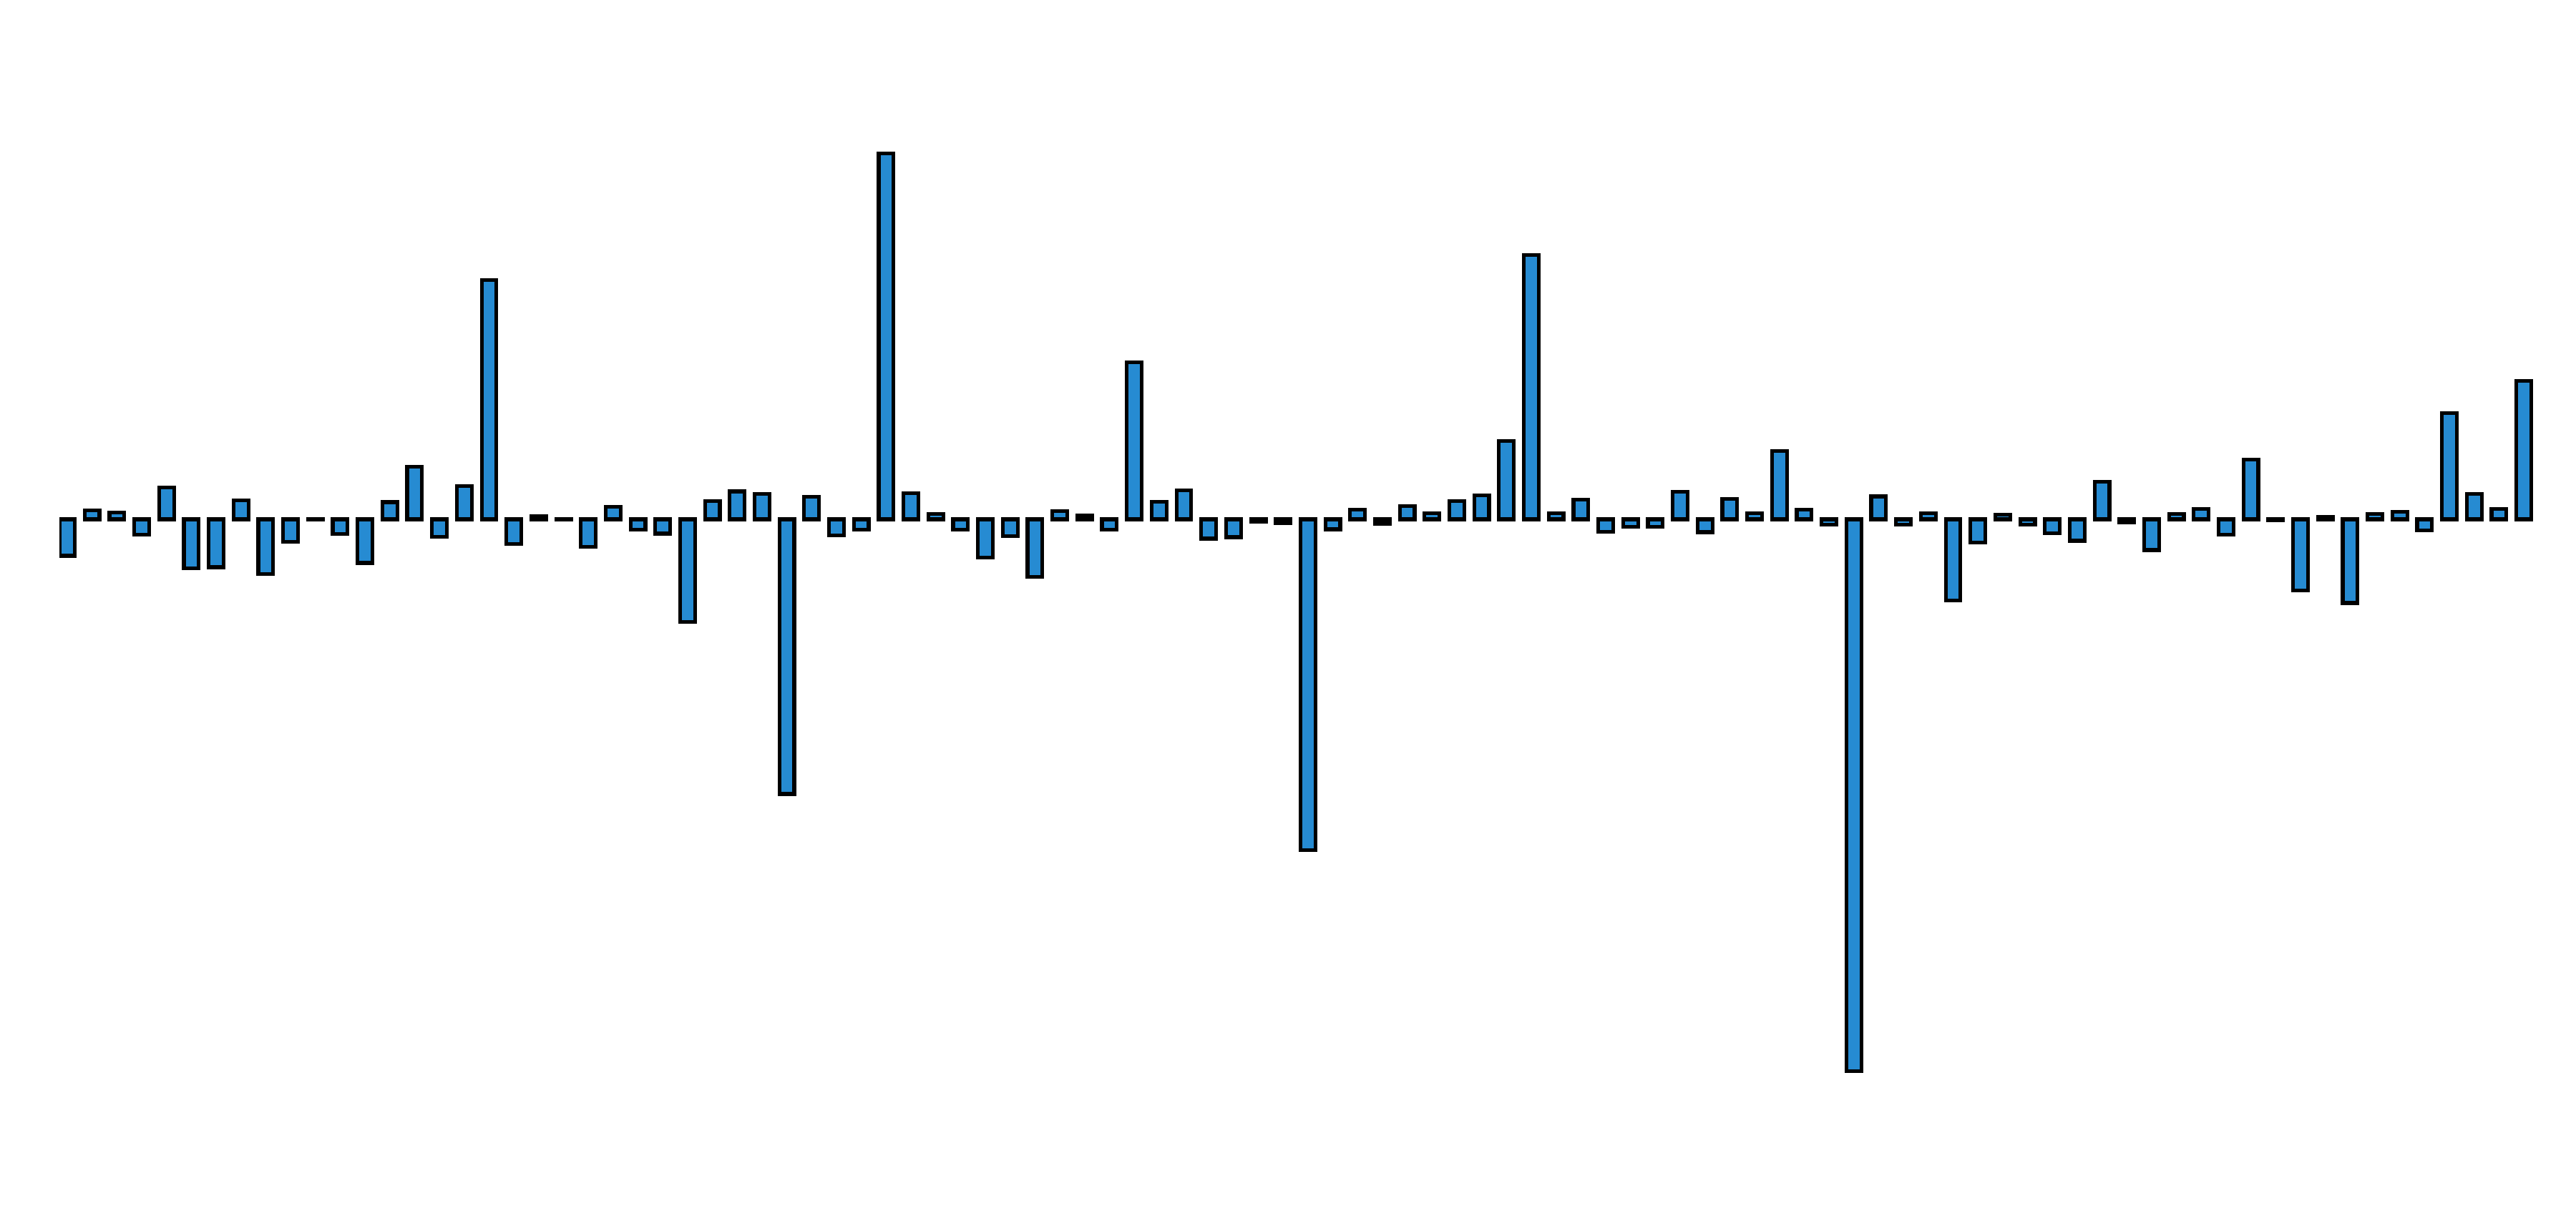
\includegraphics{LevyFlight/levy_length.pdf}
    \end{center}
    \caption{Distribution de 100 tirages aléatoire obéissant à une distribution de Lévy.
             \label{fig:levy_length}}
\end{figure}

\begin{figure}
    \begin{center}
        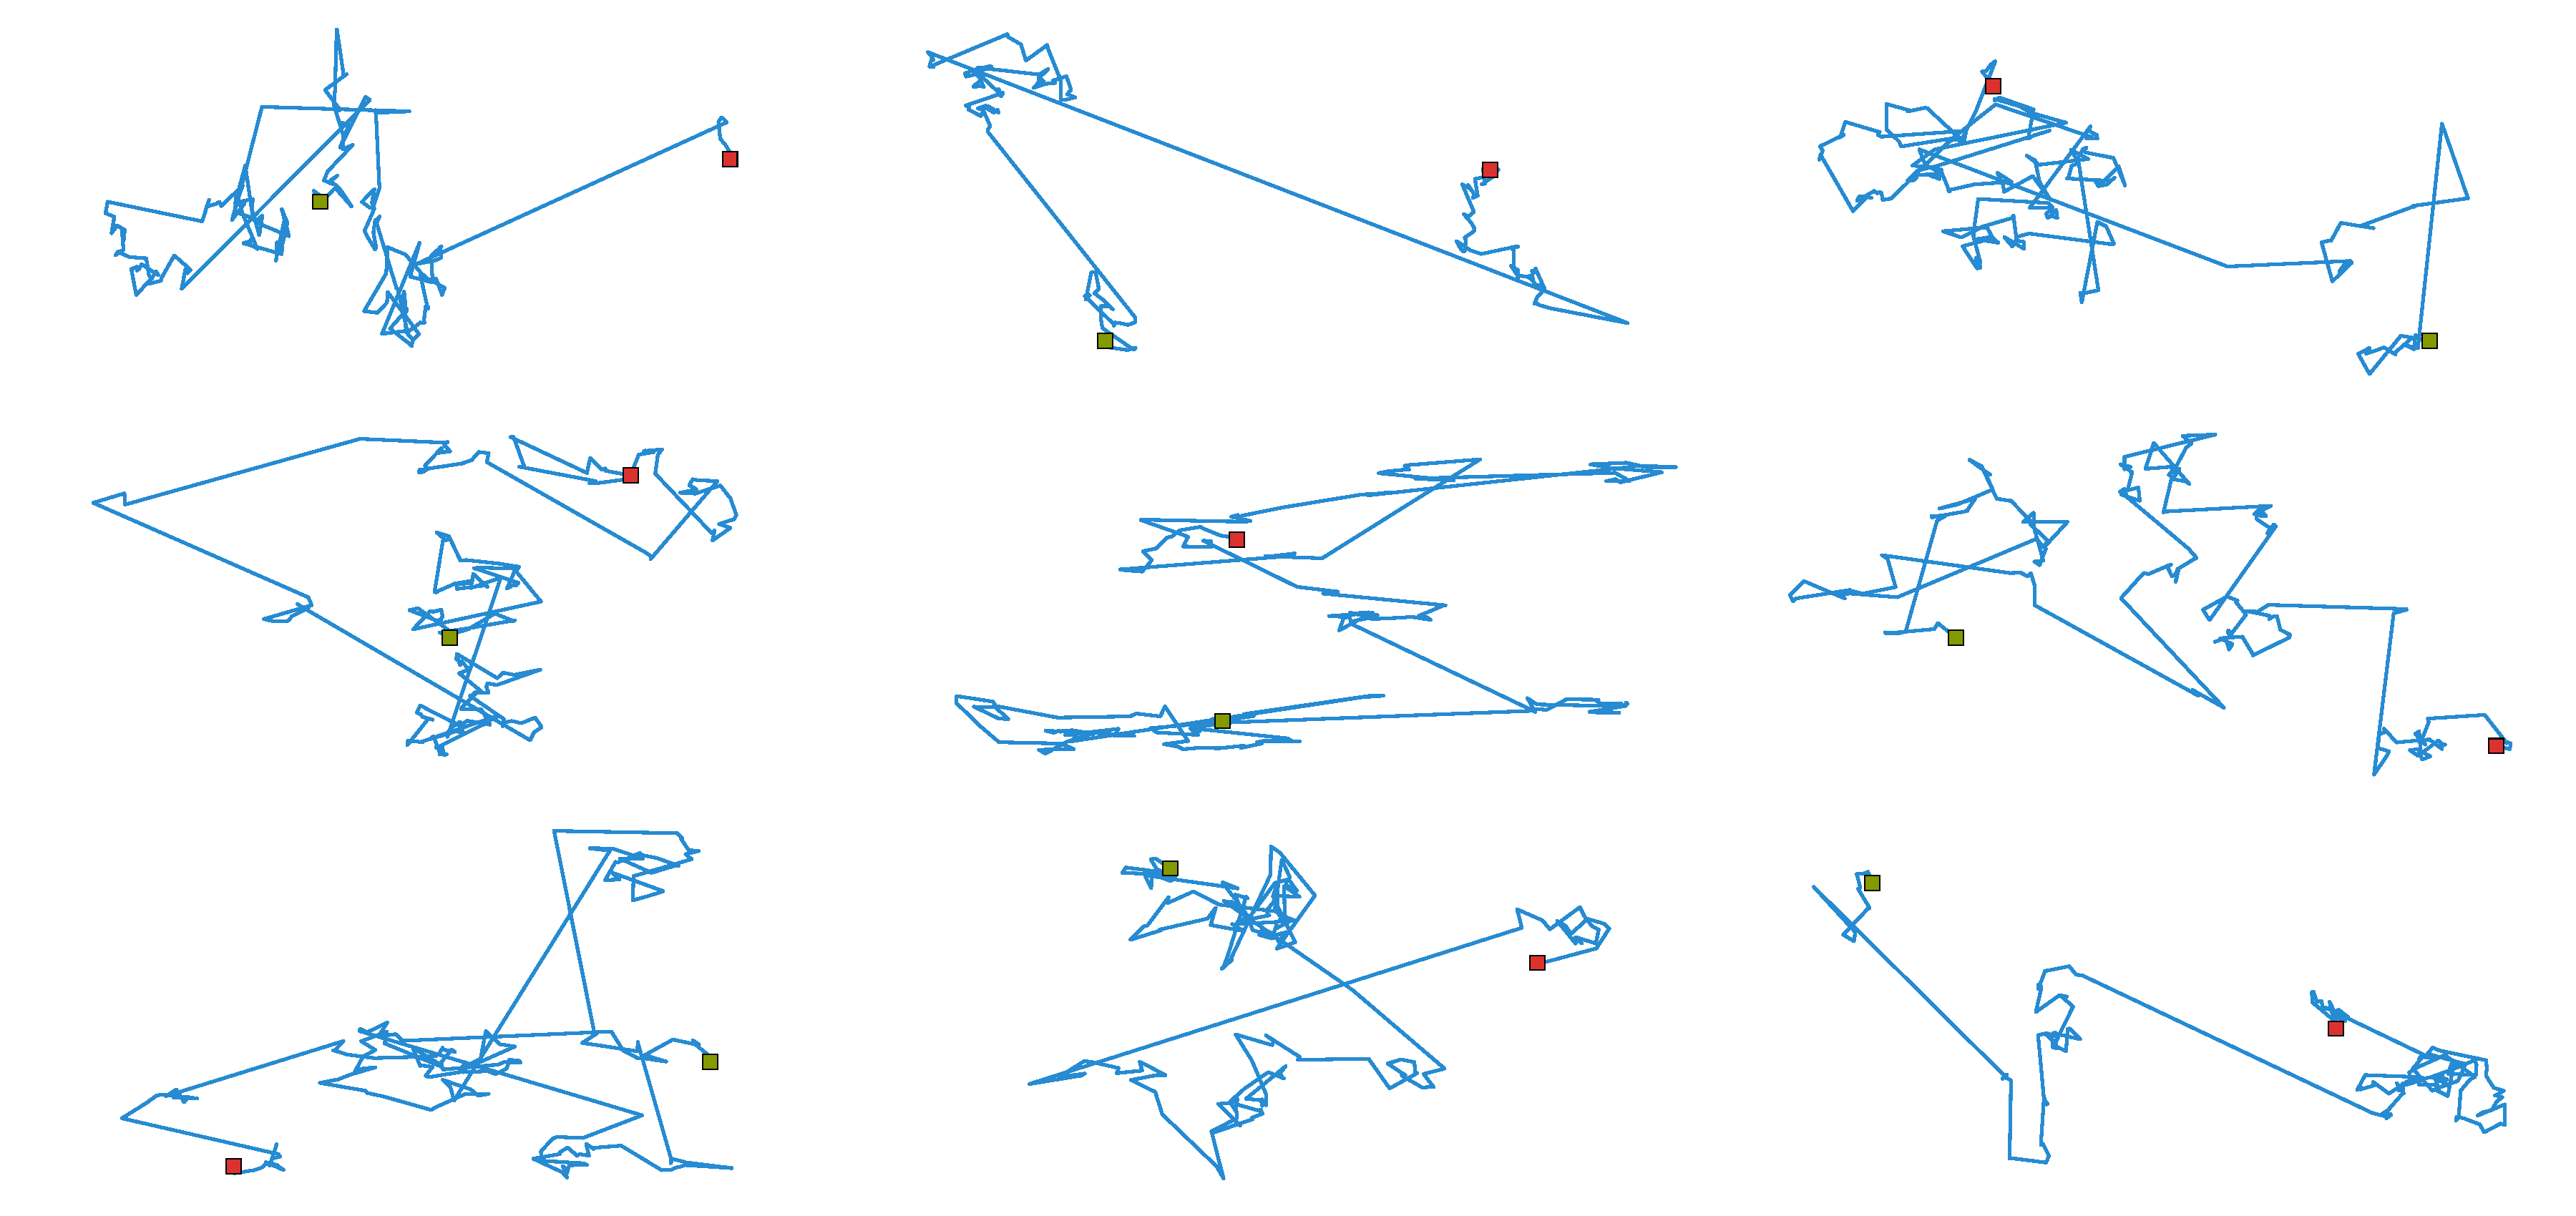
\includegraphics{LevyFlight/levy_flight.pdf}
    \end{center}
    \caption{Multiples vols de Lévy de 200 pas.
             \label{fig:levy_flight}}
\end{figure}

\begin{figure}
    \begin{center}
        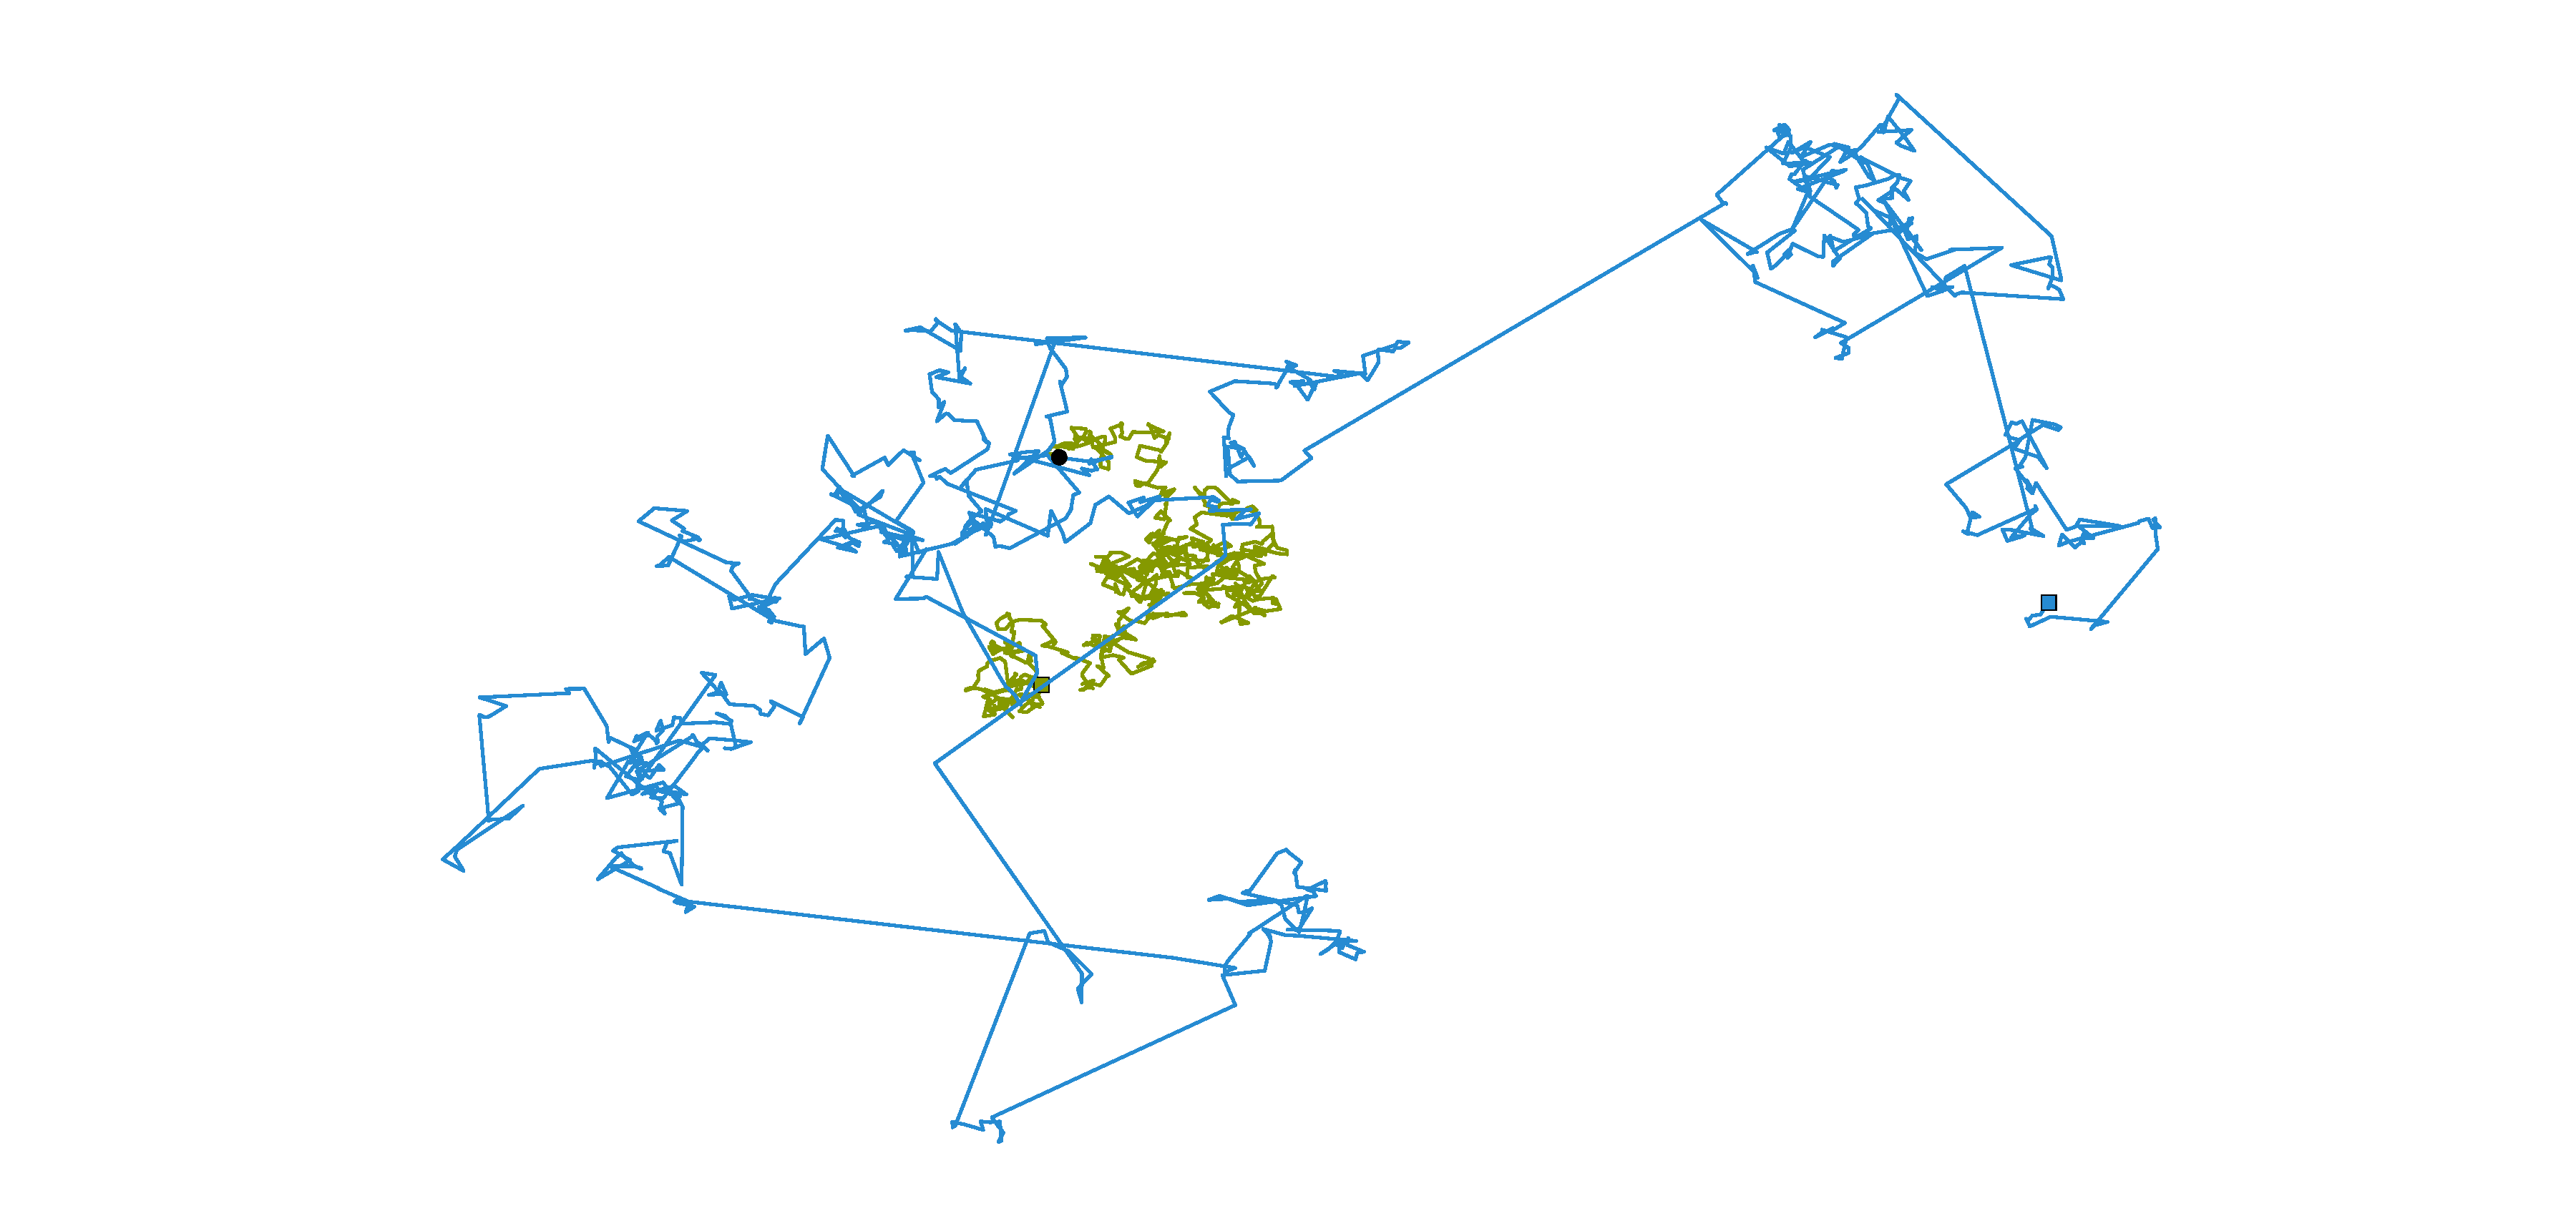
\includegraphics{LevyFlight/levy_vs_gaussian.pdf}
    \end{center}
    \caption{Mouvement browien (en vert) et vol de Lévy (en bleu) pour 200 pas aléatoires.
             \label{fig:levy_vs_gaussian}}
\end{figure}

\itodo{Ajouter des applications aux problèmes multi-objectifs}
Dans \cite{Sharma2012213}, vol de Lévy est employé pour améliorer l’algorithme ABC
pour faire une recherche locale autour de la meilleure solution actuelle. L’auteur
utilise un multiplicateur pour réduire la longueur des pas généré d’après \eqref{eq:step_len}.
De plus la meilleure solution actuelle est utilisée pour guider la recherche aléatoire et
peu être assimilé à un apprentissage. Le vol de Lévy a aussi été utilisé dans un algorithme
d’optimisation approchée, le Cuckko search. Cet algorithme est inspiré du comportement
parasitaire de la reproduction des cuculidés et a était adapté aux problèmes
multi-objectifs (\cite{Yang20131616}).
% subsubsection vol_de_lévy (end)

% - - - - - - - - - - - - - - - - - - - - - - - - - - - - - - - - - - - - - - -
\subsubsection{Apprentissage par opposition} % (fold)
\label{ssub:apprentissage_par_opposition}

La recherche par vecteur opposé (opposition-based learning) a été implémenté pour la première fois
en optimisation par \cite{Tizhoosh2005695,Rahnamayan2008155}. Il propose une méthode permettant de diversifier la
population sans connaissances à-priori.
% Opposite based learning method
\begin{Def}[OBLM~:~Opposition-Based Learning Method]\label{def:oblm}
La recherche par vecteur opposé (Opposition-Based Learning) permet de diversifier la
population sans connaissances à-priori.
Admettons un point de dimension $D$, $P(x_{1}, x_{2}, ..., x_{D})$ avec
$x_{1}, x_{2}, ..., x_{D}$ des valeurs bornées. Si $x_{i} \in [a_{i}, b_{i}]$ pour
$i = 1, 2, ..., D$ alors le point opposée est $\check{P}(\check{x_{1}}, \check{x_{2}}, ..., \check{x_{D}})$ suivant:
\[\check{x_{i}} = a_{i} + b_{i} - x_{i}\]
\end{Def}

Il est important de noter que les solutions sont comparées deux à deux par tournoi binaire, où
seule la meilleure solution entre l’initiale et son opposée est conservée. Admettons une solution
candidate $P(x_{1}, x_{2}, ..., x_{D})$ et son opposée $\check{P}(\check{x_{1}}, \check{x_{2}}, ..., \check{x_{D}})$,
alors si $f(\check{P}) \geq f(P)$ alors la solution $P$ est remplacé par $\check{P}$.
\ftodo{Illustration du tournoi binaire graphiquement}

Cette méthode a ensuite été améliorée (\cite{Rahnamayan2008155}) puis adaptée à
l’algorithme Differential evolution (DE). La méthode reprend la définition de base
mais définit plus clairement les limites et la portée de la méthode.
La méthode est utilisée durant la phase d’initialisation pour améliorer la diversité
en générant une population aléatoire de $n$ individus puis $n$ opposées.
Les solutions les plus performantes étant ensuite conservées pour obtenir une population
finale de $n$ individus.
Ensuite durant l’exécution de l’algorithme de nouvelles populations opposées sont générées.
Un coefficient $J_r$ est utilisé pour contrôler la probabilité de générer cette nouvelle
population opposée pour chaque itération.

La méthode a ensuite été testée sur un jeu de 15 fonctions de références (7 uni-modales
et 8 multi-modales). La nouvelle approche permet alors de trouver de meilleurs
résultats sur 14 des 15 fonctions. Il est aussi montré la supériorité de la
sélection par opposition par rapport au caractère aléatoire (\cite{Rahnamayan2008155,Rahnamayan2008906})
Il est aussi mis en avant que la probabilité de générer une population opposée
doit décroitre au fur et à mesure des itérations. En effet, la méthode permet de
réduire l’espace de recherche mais ralenti la convergence une fois cette intervalle
faible. Finalement il est proposé une intervalle de performance pour le coefficient si le problème
ne permet pas de déterminer un nombre fixe d’itération à-priori: $[0.1 < J_r < 0.4]$.

Cette approche a été appliquée avec succès dans le cas de l’algorithme ABC en couplage
avec un opérateur de mutation (\cite{Bi2011174}) ou encore en coopération avec une marche
aléatoire (\cite{Sharma2012213}).
Il a aussi été appliqué pour résoudre des problèmes plus complexe à objectifs multiples,
en combinaison avec un algorithme évolutionnaire (\cite{Ma201448}), ou encore avec le PSO (\cite{Gao2013114}).

Notre problème ne nous permettant pas d’avoir de connaissance à-priori, il nous est
impossible d’estimer le nombre d’itération nécessaires et l’utilisation d’un coefficient $J_r$
dynamique difficile.
% Au vu des recommandations et des applications déjà faites pour des problèmes mono-critères,
% ce coefficient sera fixé à 0.1 dans un premier temps.

\begin{figure}
    \begin{center}
        \includegraphics{abc/principe_obl.pdf}
    \end{center}
    \caption{Principe de fonctionnement de la recherche par vecteur opposée.
             \label{fig:OBL_method}}
\end{figure}
% subsubsection apprentissage_par_opposition (end)
% subsection ameliorer_l_exploration_et_l_exploitation (end)


% ------------------------------------------------------------------------------
\subsection{Prendre en compte les contraintes: quelle méthode ?} % (fold)
\label{sub:prendre_en_compte_les_contraintes_quelle_methode}
\itodo{Décrire les approches pour tacler les problèmes avec contraintes.
       Homorphous mapping, assimilation à un autre objectif (Voir Karaboga20113021)}

De nombreuses améliorations ont été proposées pour améliorer la vitesse de convergence
vers le ou les optimaux tout en évitant les optimums locaux. Cependant dans certaines
optimisation les objectifs sont dépendant de contraintes. Dans certaines conditions, il
est possible de résoudre ce problème de contrainte en bornant les variables à des solutions
réalisables mais ce n’est pas toujours possible. Lorsque ces contraintes ne peuvent pas être vérifiées
en amont de l’optimisation, il faut alors en tenir compte durant ce processus à l’aide
de méthode plus ou moins complexes.

La pénalité est l’approche la plus souvent retenue (\cite{EfrEnMezura-Montes2003}\munsure{Peut être mettre un vrai article ?}).
Cette approche demande la définition d’un facteur de pénalité qui doit être définie
avec précision pour pouvoir converger vers le/les solutions optimales qui respectent les
contraintes. Ce paramètre est dit: (i) statique si la pénalité est la somme pondérée des contraintes,
(ii) dynamique si le nombre d’itération influence le paramètre, (iii) adaptatif si l’information de la
recherche aide à sa détermination (\cite{Woldesenbet20073077}).
Enfin il est important de noter que une solution respectant toutes les contraintes sera toujours préférée
à une solution violant des contraintes même si l’évaluation des objectifs est meilleur. Il peut ainsi être
difficile d’atteindre certaines optimums\mtodo{Ceux qui sont entourés de violeur de contraintes} particulièrement
dans un espace de solutions faisables limitée.
\cite{Tsai201480} l’utilise avec deux essaims d’abeilles respectant respectivement l’algorithme
ABC et l’algorithme Bee Algorithm (BA) avec une population ajustée dynamiquement ou encore \cite{Karaboga20113021}
qui autorise des solutions ne respectant pas les contraintes à être ajoutées à la population. Ce dernier
utilise une facteur de pénalité déterminer dynamiquement évitant sa détermination empiriquement (\cite{Deb2000311}) comme
les approches plus classiques de pénalité.\mtodo{Lire cet article !!}
\\

\cite{EfrEnMezura-Montes2003} propose une méthode basée sur la sélection par tournoi binaire couplé à un mécanisme
déterministe permettant d’accepter des solutions infaisables. La probabilité de sélectionner une solution
seulement sur la performance des fonctions objectifs évolue est un paramètre adaptatif. Si durant une
certaine intervalle la déviation moyenne évolue faiblement alors la probabilité de pouvoir sélectionner
une solution uniquement sur optimalité des objectifs augmente et inversement.


\cite{Woldesenbet20073077} propose aussi une méthode ne demandant pas de paramètres supplémentaires
qui doivent être déterminé empiriquement. La première étape est de normalisé les objectifs et contraintes
grâce aux minimums et maximums à chaque itération. Ensuite une distance $d_{i}$ est
évaluée et la distance minimale est conservée. Soit $\tilde{f}$ respectivement la fonction objectif $i$ normalisée
et la somme des contraintes normalisées alors la distance s’écrit:
\begin{align}\label{eq:distance_measure}
    d_{i} = \begin{cases}
                v(x),                               \qquad & if\  r_{f} = 0\\
                \sqrt{\tilde{f}(x)^{2} + v(x)^{2}}, \qquad & otherwise\\
            \end{cases}
\end{align}
avec:
\begin{equation*}
    r_{f} = \frac{\text{Nbr de solutions faisable dans la population}}{\text{Taille de la population}}
\end{equation*}
Afin d’orienter la recherche vers un espace de solution faisables, une pénalité adaptative
est utilisé, $p_{i}(x)$, donnant un objectif final modifié de la forme: $F_{i}(x) = d_{i}(x) + p_{i}(x)$.
La population peut ainsi accepter des solutions ne respectant pas les contraintes mais
l’archive (optimisation multi-objectifs) elle n’accepte que des solutions faisables.
% subsection prendre_en_compte_les_contraintes_quelle_methode (end)


% ------------------------------------------------------------------------------
\subsection{Vers un outil d’aide à la décision par optimisation multi-objectif} % (fold)
\label{sub:vers_un_outil_d_aide_à_la_décision_par_optimisation_multi_objectif}
\itodo{Ajouter une vision globale du processus d’optimisation sous forme de graphique
      servant de résumé du chapitre.}

L’algorithme ABC modifié (Fig.~\ref{fig:abc_modifie}) comprend les même phases que l’original. La différence réside
dans le déroulement de ces phases. En effet plusieures technique présentées ci-avant
ont été implémentées afin d’améliorer l’exploitation et l’exploration de l’algorithme.
Enfin une archive par $\epsilon$-dominance est utilisé pour maintenir les solutions
non-dominées formant le front de Pareto. Cette archive est mise à jour après chaque
évaluation contrairement aux sources qui ne sont mis à jour que après chaque phase.

\begin{figure}
    \begin{center}
        \includegraphics[width=10cm, height=15cm]{abc/algorithme_complet.png}
    \end{center}
    \caption{Description globale de l’algorithme ABC modifié. Chaque phase renvois à un algorithme.
             \label{fig:abc_modifie}}
\end{figure}

Dans un premier temps l’algorithme initialise l’archive grâce aux objectifs et aux valeurs
d’epsilons puis la population est initialisé aléatoirement par OBL afin d’obtenir une meilleure diversité
(Algorithm~\ref{alg:init_phase}). Ensuite on entre dans le processus itératif
tant que la ou les conditions d’arrêts ne sont pas atteintes. Les différentes phases
sont les suivantes: (i) Phase des butineuses (Algorithm~\ref{alg:employed_phase}) qui explore l’espace de décision avec des vols de
Lévy, (ii) Phase des ouvrières (Algorithm~\ref{alg:onlooker_phase}) qui utilisent les informations acquises par les butineuses
et améliorent les sources choisies \eqref{eq:attribution_prob_to_source}, (iii) Phase des éclaireuses
(Algorithm~\ref{alg:scout_phase}) qui réinitialisent une source si elle est non fructueuse.
La longueur du vol de Lévy est définie par:
\begin{equation}\label{eq:levy_flight}
  LevyFlight = scaleFactor \times stepLength \times RandUniform(0, 1)
\end{equation}
avec $stepLength$ définie par \eqref{eq:step_len} et $scaleFactor$ fixé à 0.01.\\


% Attribution des probabilités
La probabilité de choisir une source $k$ par une ouvrière est elle définie comme:
\begin{subequations}\label{eq:attribution_prob_to_source}
  \begin{align}
    prob_{k} = &\frac{Qualite(\vec{x}_{k})}{\sum_{i=1}^{NbrSources} Qualite(\vec{x}_{i})} \\[1em]
    Qualite(\vec{x}_{k}) = &\frac{Dominance(k)}{NbrSources}
  \end{align}
  avec \emph{Dominance(k)} le nombre de source que la source $k$ domine, et \emph{Fitness}
  la qualité de la source en tenant comptes des contraintes comme définies en.
\end{subequations}

% Phase d’initialisation
\begin{algorithm}\label{alg:init_phase}
  \SetAlgoVlined
  \emph{Initialisation des sources sur l’ensemble de l’espace de décision}\;
  \For{$i \leftarrow 0$ \KwTo \ANbrSources}
  {
    \emph{Initialisation des critères pour chaque source}\;
    \For{$j \leftarrow 0$ \KwTo \ANbrCriteria}
    {
      \AComment{Génération aléatoire de la position initiale}
      $x_{ij} = x_{j}^{min} + RandUniform(0, 1) \times (x_{j}^{max} - x_{j}^{min})$\;
      avec $RandUniform$ un tirage aléatoire suivant une loi uniforme, et $x_{j}^{min}$, $x_{j}^{max}$
      respectivement le minimum et le maximum du critère $j$\;
      \vspace{1em}  % Add some space between two blocs
      \AComment{Génération de la position opposée suivant Definition~\ref{def:oblm}}
      $ \check{x_{ij}} = a_{j} + b_{j} - x_{ij}$\;
      avec $a_{j}$, $b_{j}$ respectivement les bornes inférieures et supérieurs du critère
    }
    \If{$\ASource_{i}$ respecte toutes les contraintes}
    {
      \AComment{On ajoute la source initial à l’archive}
      $\AArchive \pluseq \ASource_{i}$\;
    }
    \If{$\check{\ASource_{i}}$ respecte toutes les contraintes}
    {
      \AComment{On ajoute la source opposée à l’archive}
      $\AArchive \pluseq \check{\ASource_{i}}$\;
    }
  }
  \AComment{On ne conserve que une seule position par source}
  Mise à jour de la position des \ASources d’après Algorithm~\ref{alg:maj_phase}\;
  \caption{Initialisation des sources par OBLM (Opposite-Based Learning Method).}
\end{algorithm}

% Maj des sources
\begin{algorithm}\label{alg:maj_phase}
  \SetAlgoVlined
  Récupérer le maximum et minimum pour chaque objectif\;
  Récupérer le maximum pour chaque contrainte\;
  \For{$i \leftarrow 0$ \KwTo \ANbrSources}
  {
    Normaliser les objectifs et les contraintes avec ()\;
    Calculer la valeur de distance $\vec{d_{i}}$ en utilisant \eqref{eq:distance_measure}\;
    Calculer la pénalité $\vec{p_{i}}$ d’après ()\;
    \AComment{Attribuer les nouvelles valeurs d’objectifs aux sources}
    $\vec{F_{i}} = \vec{d_{i}} + \vec{p_{i}}$\;
    \If{$\check{\vec{F_{i}}} \succ \vec{F_{i}}$}
    {
      \AComment{On remplace la position de la source par la nouvelle}
      $\vec{x_{i}} \leftarrow \check{\vec{x_{i}}}$\;
      \AComment{On réinitialise le nombre d’échec pour la source $i$}
      $\ATrial_{i} \leftarrow 0$\;
    }
    \Else
    {
      \AComment{On incrémente le nombre d’échec pour la source $i$}
      $\ATrial_{i} \pluseq 1$\;
    }
    avec $\vec{F_{i}}$, $\check{\vec{F_{i}}}$ respectivement les vecteurs objectifs
    normalisés pour l’ancienne et la nouvelle position.\;
  }
  \caption{Mise à jour des sources}
\end{algorithm}

% Phase des butineuses
\begin{algorithm}\label{alg:employed_phase}
  \SetAlgoVlined
  \AComment{Exploration des sources par les \AEmployed}
  \For{$i \leftarrow 0$ \KwTo \ANbrSources}
  {
    Sélection aléatoire d’une source $k$ dans l’\AArchive\;
    \AComment{Génération d’une nouvelle position pour la \ASource $i$}
    \For{$j \leftarrow 0$ \KwTo \ANbrCriteria}
    {
      \begin{algomathdisplay}
        \check{x_{ij}} =%
          \begin{cases}
            x_{ij} + \ALevyFlight_{ij} \times (x_{ij} - x_{kj}) &\ \ATirage < \AMR \\
            x_{ij}                                      &\ sinon
          \end{cases}
      \end{algomathdisplay}
      avec \ATirage un nombre aléatoire uniforme (entre 0 et 1),
      \AMR un paramètre contrôlant le nombre de modifications
      et \ALevyFlight définie par \eqref{eq:levy_flight}\;
    }
    \If{aucun critère n’a été modifié}
      {
        \AComment{Sélection aléatoire d’un critère $j$ à mettre à jour}
        $\check{x_{ij}} = x_{ij} + \ALevyFlight_{ij} \times (x_{ij} - x_{kj})$\;
      }
    \If{$\ASource_{i}$ respecte toutes les contraintes}
    {
      \AComment{On ajoute la source initial à l’archive}
      $\AArchive \pluseq \ASource_{i}$\;
    }
    \If{$\check{\ASource_{i}}$ respecte toutes les contraintes}
    {
      \AComment{On ajoute la source opposée à l’archive}
      $\AArchive \pluseq \check{\ASource_{i}}$\;
    }
  }
  \AComment{On ne conserve que une seule position par source}
  Mise à jour de la position des \ASources d’après Algorithm~\ref{alg:maj_phase}\;
  \caption{Phase des butineuses.}
\end{algorithm}

% Phase des ouvrières
\begin{algorithm}\label{alg:onlooker_phase}
  \SetAlgoVlined
  \AComment{Exploitation des sources par les \AOnlookers}
  \For{$\ABee \in \AOnlookers$}
    {
      Sélection aléatoire d’une \ASource $i$ selon la probabilité
      définie par l’équation \eqref{eq:attribution_prob_to_source} (Sélection par roulette)\;
      Génération d’une nouvelle position pour la \ASource $i$ selon Algorithm~\ref{alg:employed_phase}
      (lignes 3 à 16)\;
    }
  \AComment{On ne conserve que une seule position par source}
  \AComment{Plusieurs \AOnlookers peuvent modifier la même source}
  Mise à jour de la position des \ASources qui ont été modifiées d’après Algorithm~\ref{alg:maj_phase}\;
  \caption{Phase des ouvrières.}
\end{algorithm}

% Phase des éclaireuses
\begin{algorithm}\label{alg:scout_phase}
  \SetAlgoVlined
  \For{$i \leftarrow 0$ \KwTo \ANbrSources}
  {
    \If{$\ATrial_{i} > \AMaxTrial$ }
    {
      \AComment{Exploration par les \AScouts}
      Génération de deux nouvelles positions suivant Algorithm~\ref{alg:init_phase}
      (lignes 4 à 16)\;
    }
  }
  \AComment{On conserve la meilleure solution parmi les deux nouvelles}
  Mise à jour de la position des \ASources d’après Algorithm~\ref{alg:maj_phase}\;
  \caption{Phase des éclaireuses.}
\end{algorithm}
% subsection vers_un_outil_d_aide_à_la_décision_par_optimisation_multi_objectif (end)
% section construction_d_un_outil_d_aide_à_la_decision (end)
